\chapter{Implemented Models}
In this chapter we will discuss the machine learning models that we implemented for performing the task of audio event detection. For each dataset that we used, we designed different models, hence in the next sections we discuss the models developed for each dataset starting with dataset-I.

\section{Dataset-I}

For performing the monophonic audio event detection task on this dataset, we developed two different kinds of neural network models and we also developed a k-nearest neighbor model to reproduce the baseline results available from the literature. First we performed the classification using the kNN model, then after getting our baseline results we performed the classification task using a deep neural network. Finally we used a convolutional neural network for classification. In the following, we describe these three models. For each of the models, first we provide an overview, then discuss the audio features that were used as the input to the models, and then we describe the complete classification procedure that takes place inside these models.

\subsection{k-Nearest Neighbors}

\subsubsection{System Overview}
We developed the kNN model in order to reproduce the baseline literature results. The input to our model is the audio recordings that are available in the dataset. To better understand and represent the characteristics of the sound events, spectral features - MFCCs are extracted for each frame of each audio recording. kNN is trained with such features as the input and audio class labels of 10 different types of audio events (in the form of one-hot vectors) as target/output. 

\subsubsection{Audio Features}
Motivated by the set of audio features used in \cite{salamon2014dataset}, we generate, for each audio recording, a feature set that consists of the mean, standard deviation, minimum, maximum, median, skewness and kurtosis of the MFCCs as well as the mean and standard deviation of the delta- and delta-delta-MFCCs. All these operations viz. mean, standard deviation etc. are performed over the frames of an audio recording. Initially, we extract the 25 top MFCC coefficients from a frame of a recording and then by performing the above operations, we obtain a feature set of size 275 for one audio recording. Figure~\ref{fig:feat_extract_knn_db1} shows the schematic diagram of the feature extraction process. We use Sony's WriteFeats tool for extracting MFCC coefficients from the audio recordings with the parameters mentioned in \cite{salamon2014dataset}. A review of the parameters used in MFCC extraction in  is shown in table~\ref{tab:param_mfcc_knn_db1}

\begin{figure}[!htb] 
\centering 
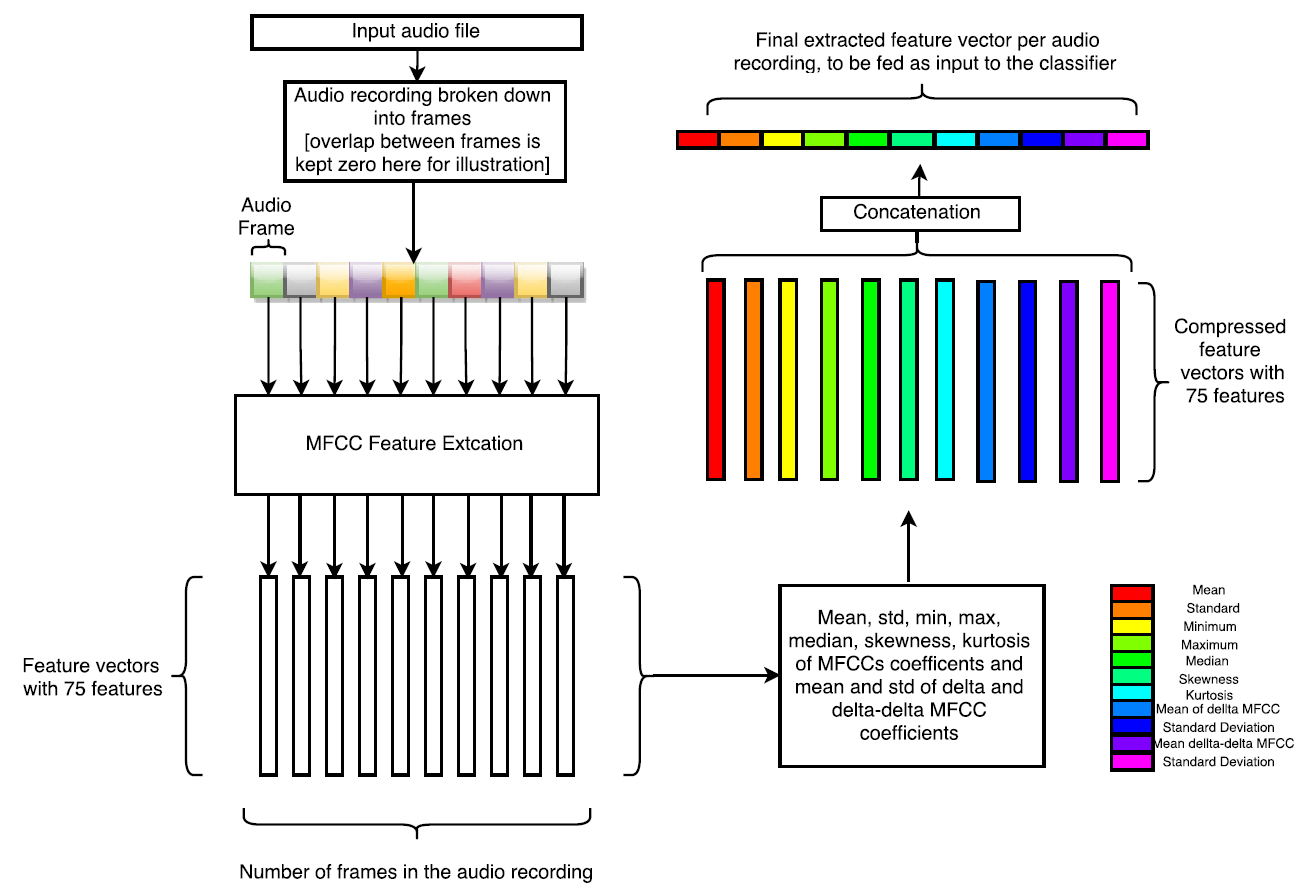
\includegraphics[width=0.95\columnwidth]{feat_extract_knn_db1}
\caption[Audio Features Extraction Schematic for kNN model]{Audio Features Extraction Schematic for kNN model}
\label{fig:feat_extract_knn_db1} 
\end{figure}

\begin{table}[tb]
\caption[Parameters for MFCC extraction]{Parameters for MFCC extraction}
\label{tab:param_mfcc_knn_db1}
\centering
\begin{tabular}{ccc}
\toprule
Parameter & Value \\
\midrule
Number of MFCC coefficients	& 25\\
Number of mel filters	& 40\\
Frame length & 23.2 (millisec)\\
Frame shift 	& 11.6(millisec)\\
Maximum allowed frequency & 22050(Hz)\\
Minimum allowed frequency & 0(Hz)\\
Windowing type & Hamming\\
Normalize mel filters (yes/no) & Yes \\
Delta MFCC context (number of neighbor frames to be included) & 21 \\
Delta-delta MFCC context & 11 \\
Channel input & 2 (channels) \\
Pre-emphasis value & 0 \\
Cepstrum lifter type & None \\
Cepstrum lifter value & 0 \\
Denoising in mel domain (yes/no) & No \\
\bottomrule 
\end{tabular}
\end{table}

\subsubsection{Classification}
We train a k-nearest neighbors classifier with $k=5$. A 10-fold cross validation experiment is run to obtain the classification performance results, where we ascertain that no two folds have audio slices/segments/excerpts from the same audio recording. The input audio feature is 275-dimensional as discussed in the previous sub-section, and the output of the classifier is a single class label, for e.g. '0' for class 'air-conditioner', '1' for 'car-horn', etc. We tried various distance measures to quantify the closeness of a data point with its neighbors, such as 'euclidean', 'cosine', 'correlation-based similarity', etc. and found that 'cosine' distance was the best distance measure in our case. Hence, we used it in obtaining the kNN results. Complete implementation of this model was performed using Matlab. The neighborhood selection method was chosen as 'exhaustive'.

\subsection{Deep Neural Network}

\subsubsection{System Overview}
Similar to the kNN model, we use spectral feature - MFCCs of the audio recordings as an input to this model. The DNN is trained with these features as input and the class labels of the audio classes as output. Posterior probabilities of audio event classes are obtained as DNN predictions. During training, the network parameters are updated to minimize a cost function C, which is a function of the posterior probabilities and target outputs. During testing, the posterior probabilities are transformed using a softmax transformation and zero-one classification error is then calculated for the testing example. Figure~\ref{fig:system_overview_db1} illustrates a high-level idea of how the system functions.

\begin{figure}[!htb] 
\centering 
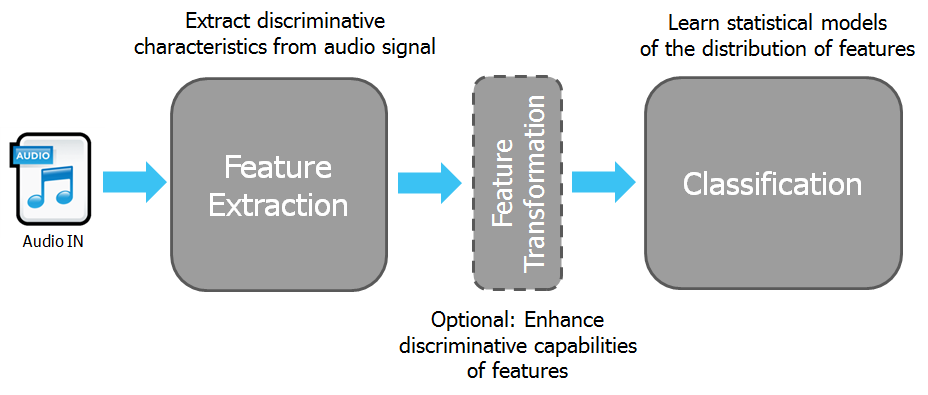
\includegraphics[width=0.95\columnwidth]{system_overview_db1}
\caption[Audio Classification Framework]{Audio Classification Framework}
\label{fig:system_overview_db1} 
\end{figure}

\subsubsection{Audio Features}
Audio features are expected to provide a reasonable representation of the time-frequency characteristics of the audio signal. MFCCs are one of the most used and successful audio features for speech recognition and events classification tasks, hence we use MFCCs as the audio features for our model. We extract the top 25 MFCC coefficients and also take the corresponding 25 delta-MFCCs and delta-delta MFCCs. This makes the input feature vector 75-dimensional. Each audio recording is broken down into constituent frames and then the mean and standard deviation of the features vectors computed over all the frames are concatenated, resulting in a vector of size 150 $(75+75=150)$. Figure~\ref{fig:feature_extraction_dnn_db1} shows the schematic for the feature extraction process. We used Sony's WriteFeat tool for extracting the MFCC features from the audio files/recordings. The parameter values used for MFCC extraction are the same as used in kNN model (see table~\ref{tab:param_mfcc_knn_db1})

\begin{figure}[!htb] 
\centering 
\includegraphics[width=0.95\columnwidth]{feature_extraction_dnn_db1}
\caption[Audio Feature Extraction Schematic - DNN]{Audio Feature Extraction Schematic - DNN}
\label{fig:feature_extraction_dnn_db1} 
\end{figure}

\subsubsection{Classification}
The neural network architecture that we developed for this dataset is inspired from \cite{gencoglu2014recognition}. There are 5 hidden layers each with 70 neurons. The final layer outputs a vector of size (10,) with the softmax probabilities for the 10 audio classes. We use sigmoid activation throughout the network, Instead of directly training the network with random initialization of the neurons, we pre-train the network using an auto-encoder pre-training technique. The details of the network architecture are presented in figure~\ref{fig:dnn_network_db1}

\begin{figure}[!htb] 
\centering 
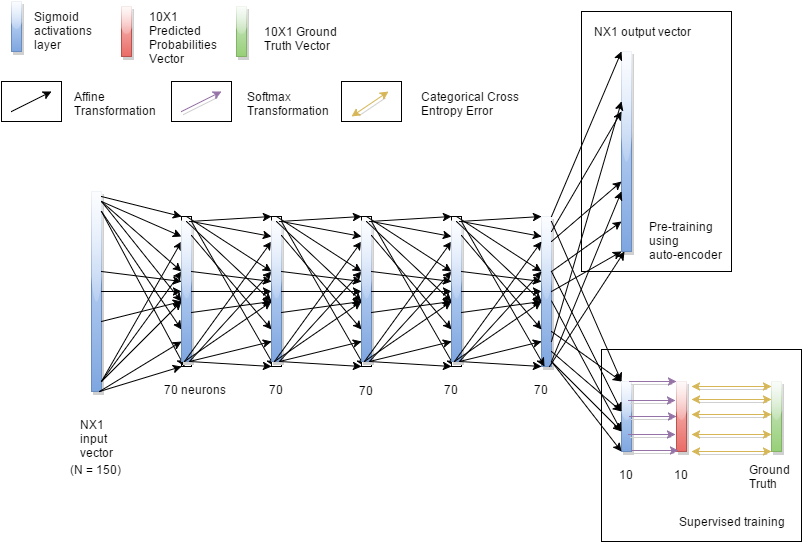
\includegraphics[width=0.95\columnwidth]{dnn_network_db1}
\caption[DNN Network Architecture]{DNN Network Architecture}
\label{fig:dnn_network_db1} 
\end{figure}

Categorical cross-entropy is used as the cost function for the training process. Zero-one error is the error-metric used for the evaluation of the performance of this classifier. The output or target audio class labels are actually one-hot vectors of size (10,). Complete implementation of the network architecture as well as the training and testing algorithm is performed using sDeePy\footnote{sDeePy provides high-level APIs on top of the basic Theano functions which makes it convenient to create, train and test neural networks.}, which is Sony's deep learning library developed in python that allows ti define, optimize and evaluate mathematical expressions involving multi-dimensional arrays efficiently.

\subsection{Convolutional Neural Network}

\subsubsection{System Overview}
In this dataset, we have most of the audio recordings sliced into audio segments of a fixed length (4 seconds). This means that all the audio recordings consist of a constant number of frames. Hence, we can imagine an audio recording as a one dimensional image, where each pixel of this image is equivalent to each frame of the audio recording. For each frame, we also compute the MFCC features as done for the kNN and DNN models. This implies that each pixel of the image can be mapped to a feature set. In other words, the one dimensional image can be represented in terms of feature maps. This manipulation facilitates us to use a CNN model on audio data just as it is used on images.

\subsubsection{Audio Features}
As used in the above two models - kNN and DNN, we used MFCCs as the audio features for this model and extracted the top 25 MFCC coefficients along with the corresponding delta-MFCCs and delta-delta-MFCCs for each frame of each audio recording. Here, we ignore the first MFCC coefficient, as it is usually done in the literature because it just represents the log of the total energy of an audio frame, hence doesn't carry any unique or useful characteristic information. After excluding the first MFCC coefficient, we obtain an input feature vector of size (74,) per audio frame. 

A single audio frame is broken down into, say, N frames and since N is constant, each audio recording can be considered as a one-dimensional vector of size (N,). Each frame, in turn, can be represented as a feature vector of size (74,). Hence we can say that each audio recording is a one dimensional image and can be represented by 74 MFCC feature maps. By this interpretation of audio recordings, it is possible to construct a CNN architecture that takes these 74 feature maps as its input. 

We used Sony's WriteFeats tool for MFCC extraction and the parameter values used in extracting the MFCCs are the same as those used in the kNN model (see table~\ref{tab:param_mfcc_knn_db1}).

\subsubsection{Classification}
We use the CNN architecture as shown in figure~\ref{fig:cnn_db1}. There is one convolutional layer with 74 different kernels of size (3,1) that convolve over the 74 respective input feature maps to produce 10 output feature maps. This layer is followed by a pooling layer, that max-pools 1 out of the 12 convolved features providing compressed representation. Finally, we have an affine/fully-connected layer that gives an output of size (10,). A subsequent softmax transformation provides the softmax probabilities for the 10 classes. We use sigmoid activation function in all the layers, throughout the network. 

\begin{figure}[!htb] 
\centering 
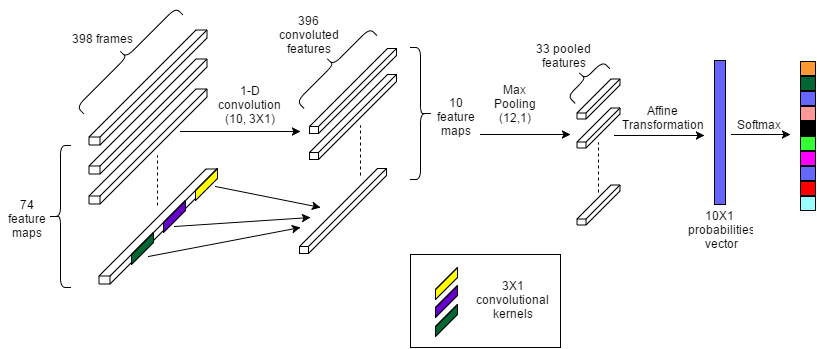
\includegraphics[width=0.95\columnwidth]{cnn_db1}
\caption[CNN Network Architecture]{CNN Network Architecture}
\label{fig:cnn_db1} 
\end{figure}

We use a learning rate of 0.0003 for training with a batch size of 50 data instances. The training is done for 1000 epochs. We do not use momentum or dropouts or any other optimization. We maintain separate training and validation data samples, with 4500 training samples and 1200 validation samples. A data sample, here, simply means an audio recording that is pre-processed into 74 feature maps.

Categorical cross-entropy is used as the cost function for the training process. Zero-one error is used as the error-metric for evaluation of the classifier performance. The output/target audio class labels are one-hot vectors of size (10,) as in the DNN model. Complete implementation of the CNN model is performed using Sony's sDeePy library.


\section{Dataset-II}
For performing the polyphonic audio event detection task on this dataset, we developed two different kinds of neural network models and we also developed a k-nearest neighbor model to reproduce the baseline results available from the literature. First we performed the classification using the kNN model, then after getting our baseline results we performed the classification task using a deep neural network. Finally we used a convolutional neural network for classification. In the following, we describe these three models. For each of the models, first we provide an overview, then discuss the audio features that were used as the input to the models, and then we describe the complete classification procedure that takes place inside these models.

\subsection{Support Vector Machine}

\subsection{Convolutional Neural Network}
